\documentclass[fleqn]{article}
% v3 2013-01-14
% v2 2008-01-17
% v1 2002\\

\usepackage{industra}
\usepackage{tabularx}

\usepackage{brochure-venturis}
\usepackage{qrcode}
\def\wLaTeX{\qrcode{https://labs.industra.space/wiki/index.php/EQ\_LaserNova63}}
\begin{document}
	


\noindent\begin{tabular}{
  @{}%	                   flush left margin
  b{.35\columnwidth}%	   logo
  @{\hspace{.03\columnwidth}}%        gap
  >{\huge\centering\color{DarkBlue}}p{.62\columnwidth}%	   headline
  @{}%                     flush right margin
}
  \raisebox{-35pt}{%
    \fontsize{60}{0}\selectfont\color{Black}\bfseries\wLaTeX}
&
  Industra Labs\\[4pt]\hrule\vspace*{7pt} 
  
  \par
  \fontsize{16}{18}\selectfont\itshape
  Laser Nova 63 User Manual
\end{tabular}

\bigskip\bigskip

\noindent\begin{tabular}{@{}
                         p{.38\columnwidth}%		blurb
		         @{\hspace{.04\columnwidth}}% 	gap
		         p{.58\columnwidth}%		quotes
		         @{}%			implicit margin
}
\sffamily\lite\fontsize{16}{18}\selectfont\raggedright 

\textit{Basic user manual for Laser Nova 63. More info can be found on our wiki  https://labs.industra.space/}
\bigskip\\
\textbf{Quick Checklist}
\begin{itemize}[noitemsep,topsep=0pt]
	\item power up the water chiller
	\item power up the laser (the Main switch)
	\item position the material inside the laser
	\item focus the laser beam
	\item set the Origin location
	\item use the LightBurn software to prepare the process
	\item power up the laser (the Laser switch)
	\item start the job
\end{itemize}
\bigskip
\textbf{Forbidden Materials}\\
\begin{itemize}[noitemsep,topsep=0pt]
	\item anything that contains chlorine (PVC, artificial leather, vinyl)
	\item Hobbyglass
	\item metal based products
	\item copper, including PCBs
\end{itemize}
\bigskip
\textbf{Miscellaneous}\\
\begin{itemize}[noitemsep,topsep=0pt]
	\item PC login: industra/industra
	\item laser chamber dimensions: 1600mm $\times$ 1000mm
\end{itemize}
\bigskip
\textbf{Support}\\
\begin{itemize}[noitemsep,topsep=0pt]
	\begin{itshape}
		\item \textbf{support.industra.space}
		\item ondrej@industra.space
		\item simon@vaizard.net
	\end{itshape}
\end{itemize}


\par\bigskip
%\vbox to7pc{\hrule\hbox to\hsize{\vrule height7pc\hfill\vrule}\hrule}

&\large
% front RH blurb
\lettrine[lines=2]{N}{ova63} is a CO2 type laser cutter with output power 120W. We use the LightBurn software to control the software.

\subsection{Notes}
\begin{itemize}[noitemsep,topsep=0pt]
	\item cleaning the optics is forbidden
	\item laser can not be used without the water chiller powered up (the machine will warn you if you forget to power it up)
\end{itemize}

\subsection{Positioning}
\begin{itemize}[noitemsep,topsep=0pt]
	\item X and Y axis can be controlled by the arrow keys on the control panel 
	\item Z axis control is accessible after pressing the \textit{Z/U} key (in the middle of arrow keys). After pressing the \textit{Z/U} key, the right arrow moves the pad down and the left arrow moves the pad up. When positioned correctly, return from the menu by pressing the \textit{ESC} button
	\item origin is set by pressing the \textit{Origin} button
	\item to move the head to the origin, quickly press the \textit{ESC} button twice
	\item movement speed of X and Y axis can be tuned by arrow keys after pressing the \textit{Speed} button
\end{itemize}

\subsection{Engraving}
There are multiple types of engraving styles available...

\subsection{Dot Mode (\textit{precision cutting})}
For cutting hard or higher depth material (8+ mm) the \textit{Dot mode} can be used. It leaves smoother and cleaner surface, but takes more time than standard cutting. It can be enabled in the cut settings window (the same where you set up laser speed and power) -- at the bottom of that window. You have to set spacing and time. The values have to be tested for each material. 18mm wood is nicely cut with spacing set to 0.10mm and time 23ms, using the 4" head.



\end{tabular}

\begin{figure}[b]
	\flushright
	\begin{itshape}
    revision: ---REVISION\_ID---, release: ---RELEASE\_ID---, build date: ---BUILDDATE---
	\end{itshape}
\end{figure}

\clearpage



%% LightBurn
\clearpage
\section{LightBurn}
Most of work with the laser happens on cards/panels Laser, Cuts and Move.
\subsection{Laser}
\setlength{\columnseprule}{0pt}
\begin{multicols}{2}\setlength{\parindent}{1em}
	\begin{itemize}
		\item \textit{Show Last Position} button --- shows a cross with a red dot representing actual position of the laser head (remember to get the actual position by pressing the \textit{Get Position} button on the \textit{Move} card)
		\item  \textit{Cut Selected Graphics} switch --- if enabled, laser will process only marked objects
		\item  \textit{Optimization Settings} button --- it is usually sufficient to keep the default values (it may only be useful to change those settings when working on large project) 
		\item  \textit{Send button} --- send the job to the laser but do not start it (can be started from the laser itself by pressing the \textit{Start/Pause} button)
	\end{itemize}
	\vfill\null
	
	\columnbreak
	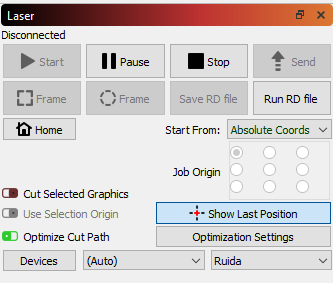
\includegraphics{imgs/lightburn_lasercard.png}
	
\end{multicols}


\subsection{Cuts}
\setlength{\columnseprule}{0pt}
\begin{multicols}{2}\setlength{\parindent}{1em}
	\begin{itemize}
		\item Fill = engraving
		\item Line = cutting
		\item  \textit{Output} checkbox --- if checked, laser will process objects with its colors, ignore them otherwise
		\item laser will process layers from top to bottom. To change priorities of some layer, use the up and down arrow buttons (marked with red arrows in the picture)
	\end{itemize}
	\vfill\null
	
	\columnbreak
	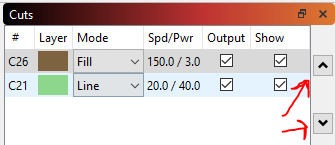
\includegraphics{imgs/laser_cutscard.png}
	
\end{multicols}

\subsection{Move}
\setlength{\columnseprule}{0pt}
\begin{multicols}{2}\setlength{\parindent}{1em}
	\begin{itemize}
		\item  \textit{Get Position} button --- get the current position of the laser head
	\end{itemize}
	\vfill\null
	
	\columnbreak
	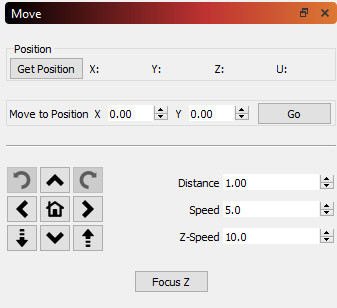
\includegraphics{imgs/laser_movecard.png}
	
\end{multicols}


%% END LightBurn %%



%% Heads and security %%
\clearpage
\section{Heads}
\setlength{\columnseprule}{0.5pt}
\def\columnseprulecolor{\color{black}}
\begin{multicols}{3}\setlength{\parindent}{1em}
	
	
\begin{center}
	\subsection{2" Cutting Head}
\end{center}
\begin{itemize}[topsep=8pt]
	\item default head for universal use
	\item capable of cutting \& engraving
	\item effective cutting of a material with depth of up to 10mm
\end{itemize}
\begin{center}
	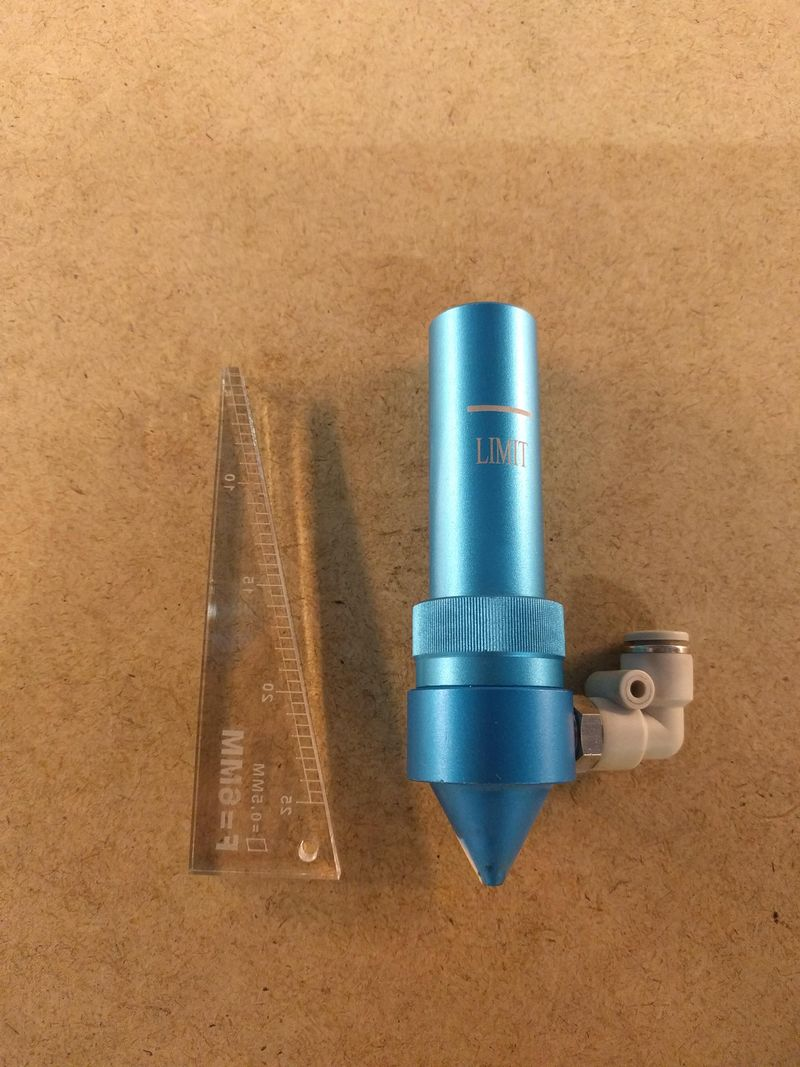
\includegraphics[width=4cm, height=5cm]{imgs/head_2.jpeg}
\end{center}


\vfill\null
\columnbreak
	
\begin{center}	
	\subsection{4" Cutting Head}
\end{center}
\begin{itemize}[topsep=8pt]
	\item intended for deeper cuts
	\item not suitable for engraving
	\item not compatible with autofocus
\end{itemize}
\medskip
\begin{center}
	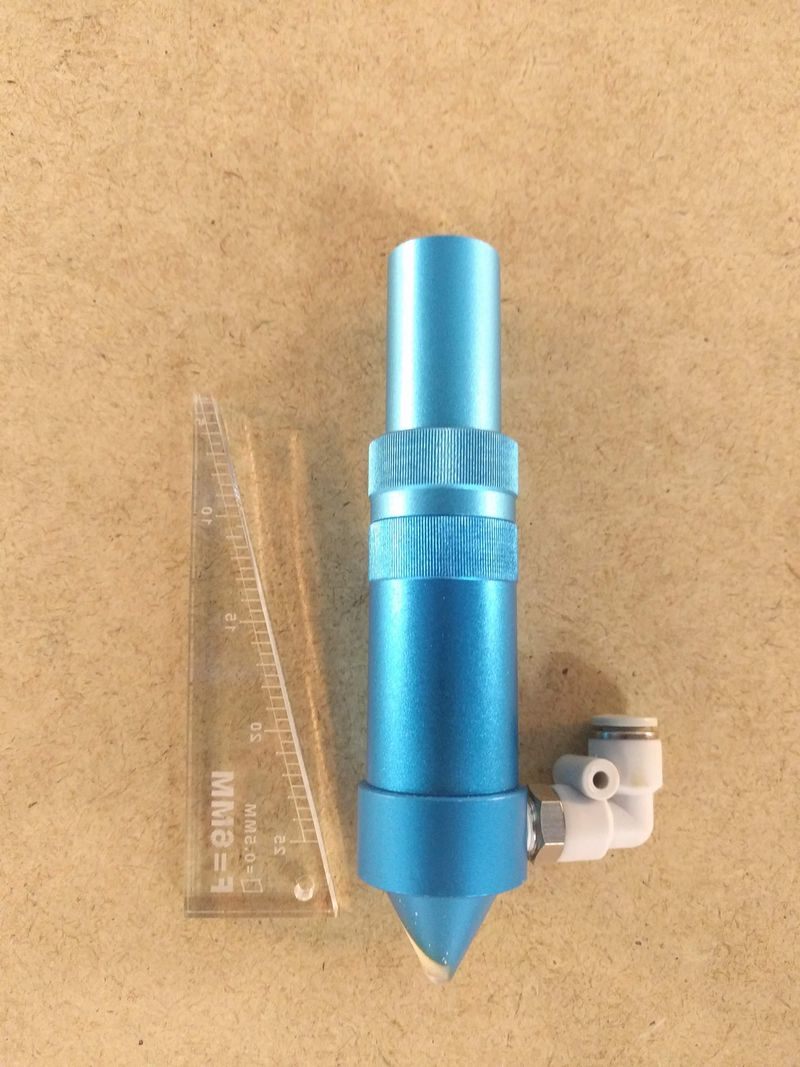
\includegraphics[width=4cm, height=5cm]{imgs/head_4.jpeg}
\end{center}
\vfill\null
\columnbreak

\begin{center}
	\subsection{High Resolution Head}
\end{center}
\begin{itemize}[topsep=8pt]
	\item engrave only
	\item requires different focus distance
\end{itemize}
\bigskip\bigskip
\begin{center}
	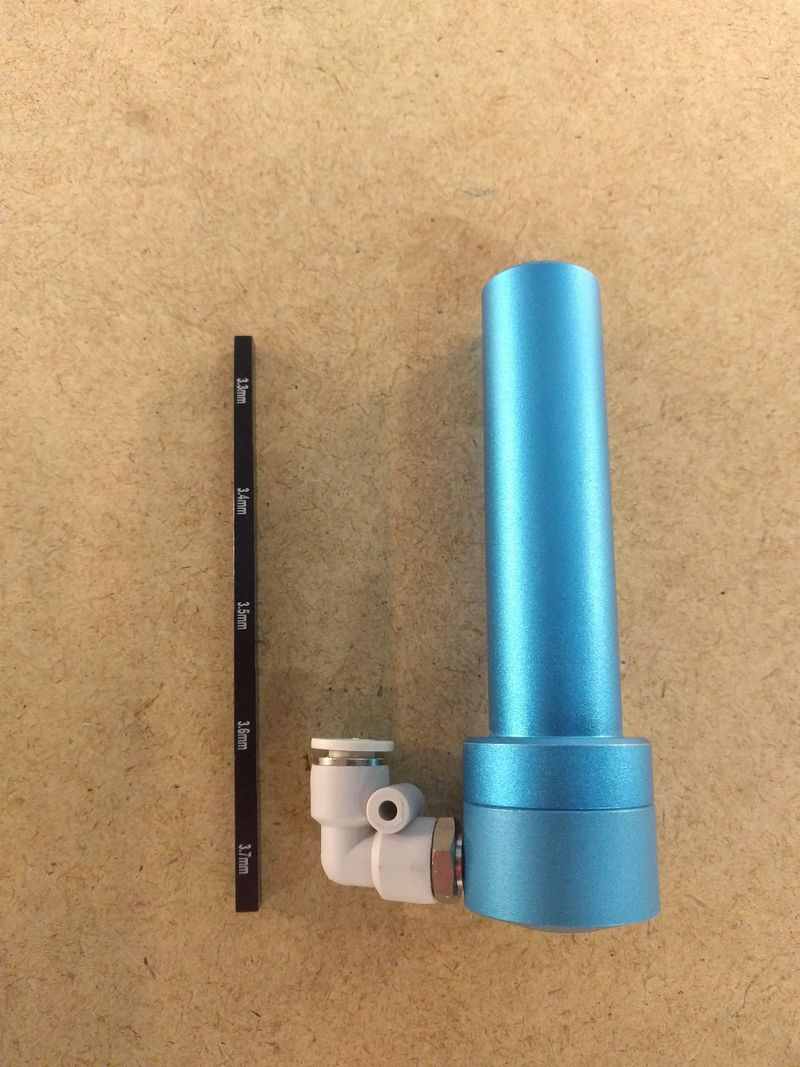
\includegraphics[width=4cm, height=5cm]{imgs/head_hr.jpeg}
\end{center}
\vfill\null
\columnbreak
\end{multicols}
	
\subsection{Replacing the Head}
You can change the head anytime, so it will suit your exact needs. Replacing the head is a straightforward process:

	\begin{itemize}[noitemsep,topsep=0pt]
		
		\item remove the air assist tube from the white part (hold the white part from the bottom using your thumb and push on the top of it, then remove the tube gently)
		\item unscrew the gold screw that holds the head and remove it
		\item insert the new head and secure the screw
		\item insert the air assist tube into the white part (pushing the top is not required this time)
		
	\end{itemize}
	
	

\section{Operation and Safety}
\begin{multicols}{2}\setlength{\parindent}{1em}
	
		\begingroup
		\color{industra-manual-darkgreen}
		\subsection{You are allowed to}
		\begin{itemize}[noitemsep,topsep=0pt]
			
			\item replace the whole laser head
			\item prepare the job in LightBurn installed on your own PC, then transfer the job to our PC and execute it from there
			
		\end{itemize}
		\vfill\null
		\endgroup
	
	\columnbreak
	
	\begingroup
		
		\color{industra-manual-darkred}
		\subsection{You are NOT allowed to}
		\begin{itemize}[noitemsep,topsep=0pt]
			
			\item connect your own PC to the laser
			\item operate the laser with any part of the case removed
			\item (re)connect any cables to the laser
			\item physically manipulate with any parts of laser (except those explicitly allowed to be manipulated, like changing the laser head)
			\item disable the air assist
			\item manipulate with the laser frequency
			
		\end{itemize}
		\vfill\null
		
		\endgroup
		\columnbreak
	

\end{multicols}

\subsection{Operational Hazards and Risks}
	\begin{itemize}[noitemsep,topsep=0pt]
	
		\item fire (ignition of the processed material)
		\item toxic or corrosive fumes
		\item laser beam irradiation (loss of eyesight, severe burn injuries) from direct and reflected beam
		\item fingers/hair/clothes can get pulled or crushed (movement of head/table with loading door opened)
		\item laser head and other parts of the machine can get damaged (curved/non-planar materials)
	
	\end{itemize}

\begin{multicols}{2}\setlength{\parindent}{1em}
	\subsection{Safety Features and Protective Equipment}
	\begin{itemize}[noitemsep,topsep=0pt]
		
		\item central stop
		\item fire extinguisher
		\item Certified laser protecting goggles
		
	\end{itemize}
	\columnbreak
	
	\subsection{Operational Malfunction}
	\begin{itemize}[noitemsep,topsep=0pt]
		
		\item job doesn't start
		\item job didn't finish
		
	\end{itemize}
		\columnbreak
	
\end{multicols}



\clearpage
\section{Materials}

\color{industra-manual-darkred}\subsection{Forbidden materials}
\color{black}


%% Use tabularx instead of tabular for easy automatic line breaks https://tex.stackexchange.com/questions/166743/automatic-line-break-in-tabular

%% Centered vertical allignment
\renewcommand{\tabularxcolumn}[1]{m{#1}}
\newcolumntype{C}{>{\Centering\arraybackslash}X}
\begin{table}[h]
	
	\centering
	\begin{tabularx}{\textwidth}{|m{10em}|l|X|}
		
		\hline
		\centering
		\textbf{Material} & \multicolumn{1}{c|}{\textbf{Danger}} & \multicolumn{1}{c|}{\textbf{Details}}                                                                                                                                                   \\ \hline
		Chlorine Based Materials (PVC/vinyl/artificial lether/...) & Toxic/dangerous fumes & Fumes produced by burning chlorine or its chemical compounds are highly toxic to people and dangerous for the equipment.                                                             \\ \hline
		Hobbyglass & Melts & Highly self healing material, which produces light spiderweb-like pollution.                                                                                                                                                                    \\ \hline
		Mirrors, PCB (copper) & Reflections & Highly reflective materials can reflect the laser beam back to its source and damage/destroy it in the process.                                                                                                                                                             \\ \hline
		ABS                                                      & Melts & ABS does not cut well in a laser cutter. It tends to melt rather than vaporize, and has a higher chance of catching on fire and leaving behind melted gooey deposits on the vector cutting grid. It also does not engrave well (again, tends to melt).
		\\ \hline
		Coated Carbon Fiber  & Fumes  & A mix of two materials. Thin carbon fiber mat can be cut, with some fraying - but not when coated.                                                                                                                                                                          \\ \hline
		PolyPropylene Foam & Fire  & Like PolyStyrene, it melts, catches fire, and the melted drops continue to burn and turn into rock-hard drips and pebbles.                                                                                                                                                  \\ \hline
		PolyStyrene Foam & Fire & It catches fire, it melts, and only thin pieces cut. This is the \#1 material that causes laser fires!   
		\\\hline                                                                                                                                                      
	\end{tabularx}
	\caption{\textit{Table source: Industra LABS and Fab Lab Oulu}}
\end{table}

\vfill


\begingroup
\color{industra-manual-darkred}
\subsection{If anything goes wrong, use the red \textbf{EMERGENCY STOP} button. For first aid, please refer to general safety instructions, esp. chapters on
	burns, inhalation of toxic fumes, laser beam irradiation and mechanical injuries.}
\endgroup
%% END heads and security%%
\begingroup




\clearpage
\generateservicelist

\clearpage
\generateservicelist


\end{document}
